

\chapter{Phenomenology of Processes}

\section[The Standard Model process \ppwbblnbb]
{The Standard Model process $\boldsymbol{\ppwbblnbb}$} \label{sec:wbbproduction}
%{The process $\boldsymbol{\mathbf{\ppwbblnbb}}$} \label{sec:wbbproduction}

The Feynman diagram depicting the full SM process \ppwbblnbb 
 along with the component vertices making it up
 are illustrated in Figure~\ref{fig:ppwbblnbbfeyn}.

%%%%%%%%%%%%%
\begin{figure}[!h]
 \center
 \caption[Feynman diagrams for \ppwbblnbb]{
  The Feynman diagram for the process
   \ppwbblnbb is illustrated below,
   and is composed from the individual vertices 
   illustrated on the left, each of which is
   described in Section \ref{sec:wbbproduction}.
 } 
\begin{tabular}{rl}
 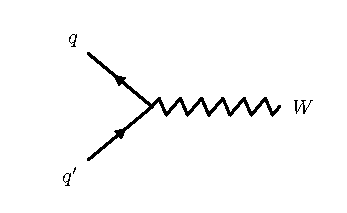
\includegraphics[width=0.3\textwidth]{/Users/rhombus/CMS/Thesis/thesis/pdfs/feyn/ppw/ppw.pdf} & 
 \multirow{3}{*}{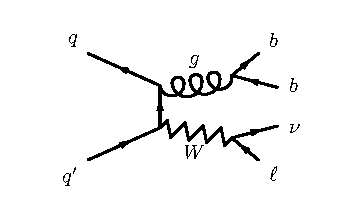
\includegraphics[width=0.6\textwidth]{/Users/rhombus/CMS/Thesis/thesis/pdfs/feyn/ppwbblnbb/ppwbblnbb.pdf}} \\
 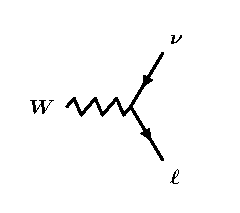
\includegraphics[width=0.3\textwidth]{/Users/rhombus/CMS/Thesis/thesis/pdfs/feyn/wln/wln.pdf} & {} \\
 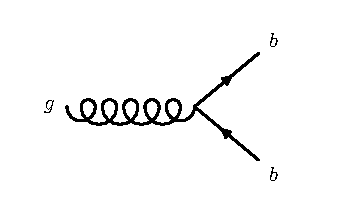
\includegraphics[width=0.3\textwidth]{/Users/rhombus/CMS/Thesis/thesis/pdfs/feyn/gbb/gbb.pdf} & {}
\end{tabular} 
    \label{fig:ppwbblnbbfeyn}
\end{figure}
%%%%%%%%%%%%%

 \subsection[\ppw]
 {$\boldsymbol{\ppw}$}

  The $W$ boson couples to all charged fermions
   and can be
   created during the collision of a quark-antiquark
   pair with a relative charge difference of $e$.
  In the proton are quarks and the most prevalent valence
   quark is the $u$.
  Therefore in a $pp$ collision,
   the channel by which most
   $W$ bosons are produced is
   via a the annihilation of a valence $u$ quark
   from one proton with 
   a $\overline{d}$ from the sea of the other,
   $u\overline{d}\rightarrow W^+$.
  Quarks of higher generation can also be found
   inside the sea as the result of gluons splitting into
   $q\overline{q}$ pairs, but all interactions
   are modified by a coefficient in the CKM matrix
   and higher generation mixing is thus suppressed.
  In this thesis, all modes of $pp\rightarrow W^\pm$ production are
   considered.

 \subsection[\wln]
 {$\boldsymbol{\wln}$}
  Just as the $W$ boson can be created by the
   collision $q\overline{q}'\rightarrow W$, 
   it can also decay as $W\rightarrow q\overline{q}'$.
  This is known as hadronic $W$ decay and
   can be a useful analysis channel for experimentalists,
   especially for decay products with energies approaching
   the \TeV scale.
  Leptonic $W$ decay, $\wln$, is also an important 
   channel for experimentalists and is the
   one considered in this analysis.
  Because leptons constitute a negligible fraction
   of the sea, the detection of leptons at high
   energy after a $pp$ collision is often a good 
   indicator of the decay of a massive gauge boson,
   $\wln$ or $Z\rightarrow \ell\overline{\ell}$.
  
  The $W$ boson is much heavier than any of the leptons
   and therefore decays with roughly equal probability
   to any of $e\nu_e, \mu\nu_\mu, \tau\nu_\tau$.
  From Table~\ref{tab:lifetimes}, tauons created
   at CMS
   subsequently decay before reaching the 
   detector, so for this analysis, the decay
   channel of the $W$ investigated is
   $\wln$ where $\ell\in e,\mu$.

 To reconstruct muons from the decay products,
  the transverse mass, $m_T$ variable is
  often used. 
 It is defined by
 $m_T^2 = m^2 + p_x^2 + p_y^2$
  where $p_i$ is the component of the momentum
  along the $i$ axis, and in the case of 
  a massive particle decaying to two massless
  particles, can be rewritten as
\begin{equation}
 m_T^2=2p_{T,1}p_{T,2}\left(1-\cos\phi\right)
\end{equation}
  where $\phi$ is the angle between the particles
  and $p_{T,j}$ is the component of the
  momentum of the particles in the transverse plane.

 In the decay of a $W$ boson, a neutrino 
  is produced, but can not be detected.
 The CMS detector is designed to
  capture the energy from all of the other 
  particles produced in a collision,
  so neutrinos are accounted for as \met.
 The variable \met is the
  transverse component of the negative
  vector sum of all of the 
  energy identified as having come from a particular
  interaction vertex,
  known as the primary vertex.
 Therefore the transverse mass of the $W$
  boson is 
\begin{equation}\label{eq:transversemass}
 \left(m_T^W\right)^2=2p_{T}^\ell\met\left(1-\cos\phi\right)
\end{equation}
  where $\phi$ is the angle between the lepton
  and \met.

 \subsection[\gbb]
 {$\boldsymbol{\gbb}$}
  Because quarks couple strongly to gluons
   and $q\overline{q}'\rightarrow W$ has been shown to be
   an important production channel in $pp$ collisions,
   it is possible for one of the
   initial state quarks to radiate a gluon.
  This is called initial state radiation, ISR,
   and if the gluon is produced with enough energy,
   it is capable of splitting to a quark-antiquark pair.
  In particular, a $g\rightarrow b\overline{b}$ vertex
   can be added to either of the incoming quarks to 
   form \ppwbblnbb.
  
  
%
% \subsection{b-jets}
%  quarks, jets/hadronization \\
%  heavy flavor - b quarks \\
%  displaced vertices
%

\section[The Standard Model process \ppzgnng]
        {The Standard Model process $\boldsymbol{\ppzgnng}$} \label{sec:znngproduction}

The Feynman diagram depicting the full SM process \ppzgnng 
 along with the component vertices making it up
 are illustrated in Figure~\ref{fig:ppzgnngfeyn}.

%%%%%%%%%%%%%
\begin{figure}[!h]
 \center
 \caption[Feynman diagrams for \ppzgnng]{
  The Feynman diagram for the process
   \ppzgnng is illustrated below,
   and is composed from the diagrams 
   illustrated on the left, each of which is
   described in Section \ref{sec:znngproduction}.
 } 
\begin{tabular}{rl}
 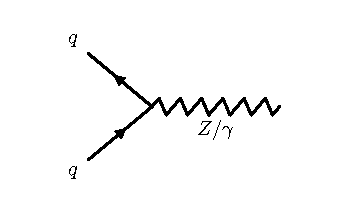
\includegraphics[width=0.3\textwidth]{/Users/rhombus/CMS/Thesis/thesis/pdfs/feyn/ppzsg/ppzsg.pdf} & 
 \multirow{3}{*}{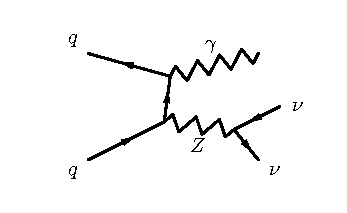
\includegraphics[width=0.6\textwidth]{/Users/rhombus/CMS/Thesis/thesis/pdfs/feyn/ppzgnng/ppzgnng.pdf}} \\
 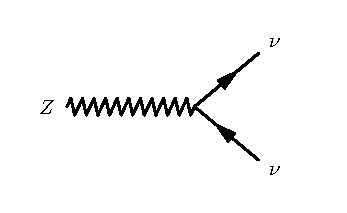
\includegraphics[width=0.3\textwidth]{/Users/rhombus/CMS/Thesis/thesis/pdfs/feyn/znn/znn.pdf} & {} \\
 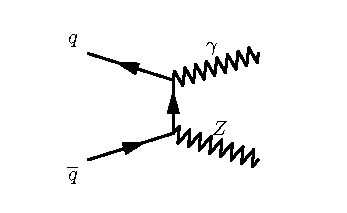
\includegraphics[width=0.3\textwidth]{/Users/rhombus/CMS/Thesis/thesis/pdfs/feyn/ppzg/ppzg.pdf} & {} 
\end{tabular} 
    \label{fig:ppzgnngfeyn}
\end{figure}
%%%%%%%%%%%%%

 \subsection[\ppzsg]
 {$\boldsymbol{\ppzsg}$}

 Similar to the $W$ boson, the $Z$ boson and the photon can
  also each be produced via the collision of quarks in
  the process $q\overline{q} \rightarrow Z/\gamma$.
 Unlike interactions with the $W$ boson, 
  interactions with $Z/\gamma$ conserve parity invariance
  and do not transport charge.
 Any interaction which can happen as mediated
  by a photon can also happen with the exchange
  of a $Z$ boson, but for collisions at $\sqrt{s}<M_Z = 90$ \GeV,
  the $Z$ can not be made on-shell.
 In this low energy regime $\gamma$ exchange dominates,
  but in 2015, the LHC ran at $\sqrt{s}=13$ \TeV
  and the relative mass difference between the $Z$ and the $\gamma$
  played a negligible role in their relative rates of production. 


 \subsection[\znn]
 {$\boldsymbol{\znn}$}

 The only particle which the $Z$ boson can couple to 
  but the photon can not is the neutrino.
 At $\sqrt{s}=13$ \TeV, the mass differences between
  the five lightest flavor of quark and the six 
  leptons are negligible and the $Z$ boson
  can decay into any kinematically allowed pairs,
  $Z\rightarrow f\overline{f}$.
 Including the three color possibilities
  for each quark, these are $3\times 5 + 6 = 21$ final states,
  each of which has roughly the same branching
  fraction. 
 Therefore only approximately $\sfrac{2}{7}$ of $Z$
  decays happen in the leptonic channel $Z\rightarrow \ell \overline{\ell}$.
  and of these decays, approximately $\sfrac{2}{3}$ happen
  as $Z\rightarrow \nu\overline{\nu}$.

 \subsection[\ppzgnng]
 {$\boldsymbol{\ppzgnng}$}

 With the photon coupling only to 
  electrically charged particles,
  the only place where a vertex
  containing a photon could be attached to
  either of the upper two left diagrams
  in Figure~\ref{fig:ppzgnngfeyn}
  is on one of the quarks.
 Photons are massless and therefore stable
  and so are a final state observable.
 Like the gluon in $\ppwbblnbb$,
  the photon is an example of ISR.
 In the CM frame of the colliding $q\overline{q}$,
  which is approximately the lab rest frame
  for colliding beams of equal energy as is the
  case at the LHC,
  conservation of momentum dictates
  that the $Z$ boson and photon should have 
  equal and opposite momenta.

 Unlike any of the other fermions, 
  neutrinos are electrically neutral
  and therefore only interact via
  the weak force. 
 So while the cross sections for
  most fermion-fermion interactions involve
  contributions from the comparatively stronger
  electromagnetic and strong forces,
  the neutrino cross section contains
  contributions from only the $W$ and $Z$
  bosons at tree-level and is
  much smaller than that of the charged fermions.
 This makes the detection of neutrinos very difficult in general,
  and impossible to do with present technology
  given the extreme backgrounds present
  in a collider setting.
%  and the Ice Cube dedicated neutrino detector encompasses
%  a cubic kilometer.
  
 In the case where the ISR photon is recoiling
  against a $Z$ boson which decays
  to neutrinos, 
  no direct detection of the $Z$ boson or of
  its decay products is possible,
  leaving only the photon visible in the final state.
 This is called the monophoton signature,
  where a photon is observed recoiling against
  apparently nothing, and while the
  monophoton signature is predicted to be
  observed as a result of SM process as in $\ppzgnng$,
  if the observed monophoton cross section is measured to be higher 
  than predicted, it could also be an indicator of physics beyond the SM (BSM).
 Specifically, the monophoton signature used in searches for dark matter.


 \section[Beyond the Standard Model: \ppgdm]
 {Beyond the Standard Model: $\boldsymbol{\ppgdm}$}

%%%%%%%%%%%%%
\begin{figure}[!h]
 \center
 \caption[Feynman diagrams for dark matter monophoton production]{
  Feynman diagrams for the DM process
   \ppgdm using simplified models
   are illustrated below.
  On the left is the $U(1)$ gauge
   model in which DM production
   is mediated by $M$ which can 
   be either vector or axial-vector,
   \ppgmgcc.
  On the right is the diagram for 
   DM production using an 
   EFT model of the $\gamma\gamma\chi\overline{\chi}$
   coupling, for the total process
   \ppggcc.
 } 
 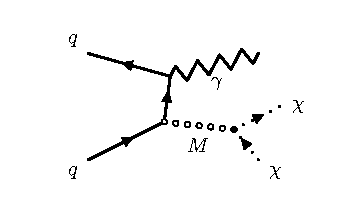
\includegraphics[width=0.4\textwidth]{/Users/rhombus/CMS/Thesis/thesis/pdfs/feyn/ppxg/ppxg.pdf}
 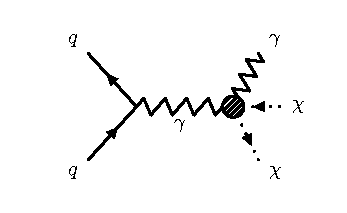
\includegraphics[width=0.4\textwidth]{/Users/rhombus/CMS/Thesis/thesis/pdfs/feyn/ppgx/ppgx.pdf}
    \label{fig:ppxgfeyn}
\end{figure}
%%%%%%%%%%%%%

 The existence of particle dark matter
  is well motivated, and the simplified
  model theories of DM used in this thesis allow
  for interactions which can result in
  the monophoton signature.
 One of the classes of models considered is a $U(1)$
  gauge theory in which $\chi\overline{\chi}$
  is produced via a vector or axial-vector mediator $M$
  which couples to quarks. 
 The tree-level process in this model which leaves
  a  monophoton signature 
  is illustrated on the left of
  Figure~\ref{fig:ppxgfeyn}, and the
  relevant parameters governing
  the cross section of this interaction are
  the masses of the two particles, $m_\chi$
  and $m_M$, and the strengths of the couplings
  between $M$ and quarks, $g_{Mq}$,
  and between $M$ and DM, $g_{M\chi}$.
 An EFT describing the four-point interaction
  vertex $\gamma\gamma\chi\overline{\chi}$ is also
  considered and illustrated on the right side of
  Figure~\ref{fig:ppxgfeyn}.
 In this theory, the coupling is a function
  of two parameters, $k_1$ and $k_2$,
  and is moderated by a mass scale, $\Lambda$.
 The other parameter in the EFT is $m_\chi$,
  and by measuring the cross section for
  \ppgdm in comparison with the SM prediction,
  estimations or limits can be set on 
  the parameters used in either of these
  two models.
  
